Vampire is the first theorem prover to implement \newcnf{}. We extended Vampire's implementation of \newcnf{} to enable support for \folb{} formulas. This extension comprised about 500 lines of C++ code. %It will be included in the forthcoming official release of Vampire.

% Our implementation is available at \url{www.cse.chalmers.se/~evgenyk/fool-cnf-experiments/} and will be included in the forthcoming official release of Vampire.

In this section we present experimental results obtained by running Vampire on \folb{} problems. In particular, we compare performance of Vampire with the extended \newcnf{} algorithm and with the translation of \folb{} formulas to FOL presented in~\cite{FOOL}. In the sequel, by Vampire we will mean its version with the extended \newcnf{}. We will write \oldcnfVampire{} for its version with the translation of \folb{} formulas to FOL and enabled \folb{} paramodulation.

For our experiments we used two sets of problems. The first set is taken from our previous work~\cite{VampireAndFOOL} on the implementation of \folb{} in Vampire. The seconds set consists of problems from the SMT-LIB library~\cite{SMT-LIB}, a corpus of benchmarks for satisfiability modulo theory (SMT) solvers.

In our previous work~\cite{VampireAndFOOL} we experimented with our initial implementation of \folb{} in Vampire. For that experiment we generated two set of \folb{} problems.
\begin{enumerate}
  \item Problems from the higher-order part of the TPTP library~\cite{TPTP} that can be directly expressed in \folb{}. We translated these problems from the TPTP language of higher-order logic to the modification of TPTP that supports \folb{}.
  \item Problems about properties of (co)algebraic datatypes generated by the Isabelle theorem prover~\cite{Isabelle} to be checked by SMT solvers. We translated these problems from the SMT-LIB~2 language to TPTP using the SMTtoTPTP tool~\cite{SMTLIB2TPTP}.
\end{enumerate}

For this work we used the second set of problems and run Vampire in the matching experimental setup. We did not use the first set in this work~--- problems in this set are easy and all of them were already solved by Vampire before.

Our results are summarised in Tables~\ref{table:isabelle-results}--\ref{table:smt-lib-results2} and discussed below. 

\subsection[Experiments with Algebraic Datatypes Problems]{Experiments with Algebraic\\Datatypes Problems}
The set of problems about (co)algebraic datatypes generated by Isabelle and translated by us to the TPTP syntax contains 152 problems. All of them use \folb{} features: boolean variables occurring as formulas, formulas occurring as arguments to function and predicate symbols, and \ITE\ expressions. None of the 152 problems use \LETIN\ expressions.

We run Vampire twice on each problem: once using the option \verb'--mode' \verb'casc', and once using \verb'--mode casc_sat'. Both times the \ITE\ expansion threshold was set to 3, the default value. For each problem, we recorded the fastest successful run of Vampire. \iffalse The experiments were run on a MacBook Pro with a 2,9 GHz Intel Core i5 and 8 Gb RAM, and using the time limit of 60 seconds per problem.\fi We then compared Vampire with the results of \oldcnfVampire, CVC4~\cite{CVC4} and Z3~\cite{Z3}, taken from~\cite{VampireAndFOOL}. 

Table~\ref{table:isabelle-results} summarises the results of our experiments on these 152 problems. Vampire solved the largest number of problems, and all problems solved by \oldcnfVampire\ were also solved by Vampire. Figure~\ref{fig:isabelle-diagram} shows the Venn diagram of the sets of problems solved by Vampire, CVC4 and Z3, where the numbers denote the numbers of solved problems. Compared to \oldcnfVampire, Vampire solved one more problem that was previously only solved by Z3 and 18 more problems, not solved by either Z3 or CVC4. This is significant because the problems were tailored for SMT reasoning. Based on our experimental results we observe that our implementation of the extended \newcnf{} improved the performance of Vampire on this set of problems.

\begin{table}[tb]
  \caption{Runtimes in seconds of provers on the set of 152 algebraic datatypes problems.}
  \begin{center}
  \begin{tabular}{lrr}
    \hline Prover & Solved & Total time on solved problems \\ \hline
    Vampire & 78 & 19.416 \\
    \oldcnfVampire & 59 & 26.580 \\
    Z3 & 57 & 4.291 \\
    CVC4 & 53 & 25.480
  \end{tabular}
  \end{center}
  \label{table:isabelle-results}
\end{table}

\begin{figure}[tb]
  %\vspace{-0.3em}
  \centering
  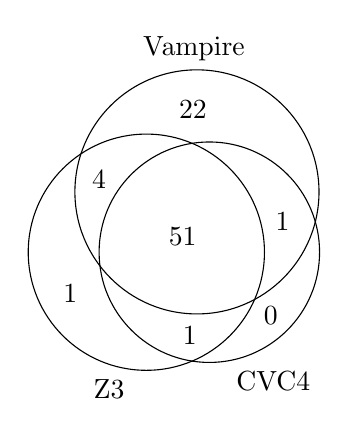
\begin{tikzpicture}
    \draw (0,0) circle (1.5cm);
    \draw (50:1cm) circle (1.55cm);
    \draw (0cm:0.8cm) circle (1.4cm);
    \node at (0.8cm:0.5cm) {$51$}; %
    \node at (-2.2cm:1.2cm) {$1$};
    \node at (1cm:-1.1cm) {$1$};
    \node at (-2cm:-1.1cm) {$4$};
    \node at (-3.8cm:-1.9cm) {$22$}; %
    \node at (-0.95cm:1.775cm) {$0$}; %
    \node at (0.45cm:1.775cm) {$1$}; %
    \node at (2.7cm:2.65cm) {Vampire};
    \node at (-3.7cm:1.8cm) {Z3};
    \node at (-1.6cm:2.3cm) {CVC4};
  \end{tikzpicture}
  \vspace{-0.3em}
  \caption{Venn diagram of the subsets of the algebraic datatypes problems, solved by Vampire, CVC4 and Z3.}
  \label{fig:isabelle-diagram}
\end{figure}

\subsection{Experiments with SMT-LIB Problems}

\folb{} can be regarded as a superset of SMT-LIB core logic and problems of SMT-LIB core logic can be directly expressed in \folb{}. The language of \folb{} extends the SMT-LIB core language with local function definitions, using \LETIN\ expressions defining functions of arbitrary, and not just zero, arity. A theorem prover that supports \folb{} can be straightforwardly extended to read problems written in the SMT-LIB syntax.

For this experiment we used problems in quantified predicate logic with uninterpreted functions stored in the UF subspace of the SMT-LIB library. These problems are written in the SMT-LIB~2 syntax. In order to read them we implemented a parser for a sufficient subset of the SMT-LIB~2 language in Vampire. The implementation comprised about 2,500 lines of C++ code. 

In this experiment we evaluated performance of Vampire, \oldcnfVampire, and CVC4 on unsatisfiable problems of the UF subspace. Each problem in the SMT-LIB library is marked with one of the statuses \verb'sat', \verb'unsat' and \verb'unknown'. A problem is marked as \verb'sat' or \verb'unsat' when at least two SMT solved proved it to be satisfiable or unsatisfiable, respectively. Otherwise, a problem is marked as \verb'unknown'. In order to filter out satisfiable problems we run Vampire, \oldcnfVampire, and CVC4 on the problems marked as \verb'unsat' and \verb'unknown' and then recorded the results on the problems that were proven unsatisfiable by at least one prover. That gave us 2596 problems.

The problems in this set use \ITE\ expressions, \LETIN\ expressions that define constants, and formulas 
occurring as arguments to equality. None of the problems use quantifiers over the boolean sort.

We run Vampire twice on each problem: once with naming of \LETIN\ expressions, and once with inlining. Both times the \ITE\ expansion threshold was set to 3, the default value. In both runs we also used the option \verb'--mode casc'. For each problem, we recorded the fastest successful run of Vampire. We run \oldcnfVampire\ once on each problem with the option \verb'--mode casc'.

\begin{table}[tb]
  \caption{Runtimes in seconds of provers on the set of 2596 unsatisfiable SMT-LIB problems.}
  \begin{center}
  \begin{tabular}{lrr}
    \hline Prover & Solved & Total time on solved problems \\ \hline
    Vampire & 2329 & 11,057.374 \\
    CVC4 & 2084 & 26,309.466 \\
    \oldcnfVampire & 2060 & 14,189.568
  \end{tabular}
  \end{center}
  \label{table:smt-lib-results2}
\end{table}

\begin{figure}[tb]
  \centering
  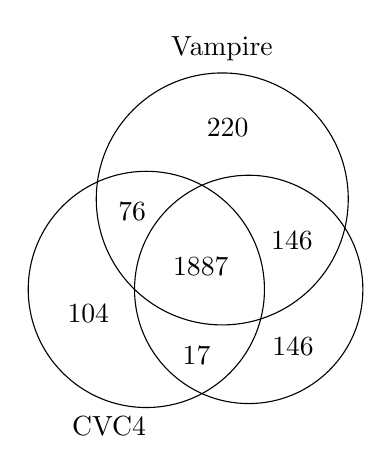
\begin{tikzpicture}
    \draw (0,0) circle (1.5cm);
    \draw (50:1.5cm) circle (1.6cm);
    \draw (0cm:1.3cm) circle (1.45cm);
    \node at (0.8cm:0.75cm) {$1887$}; %
    \node at (-1.85cm:1.05cm) {$17$};
    \node at (0.8cm:-0.8cm) {$104$};
    \node at (-2.8cm:-1.0cm) {$76$};
    \node at (-4.1cm:-2.3cm) {$220$}; %
    \node at (-0.75cm:2cm) {$146$}; %
    \node at (0.65cm:1.95cm) {$146$}; %
    \node at (2.55cm:3.2cm) {Vampire};
    \node at (-3.7cm:1.8cm) {CVC4};
    \node at (-1.6cm:2.4cm) {\oldcnfVampire};
  \end{tikzpicture}
  \vspace{-0.3em}
  \caption{Venn diagram of the subsets of the unsatisfiable SMT-LIB problems, solved by Vampire, \oldcnfVampire\ and CVC4.}
  \label{fig:smt-lib-newcnf-diagram}
\end{figure}

Table~\ref{table:smt-lib-results2} summarises the results of our experiments on the SMT-LIB problems. These results are obtained on the StarExec compute cluster~\cite{starexec} using the time limit of 5 minutes per problem. Vampire solved the largest number of problems and was the fastest among the provers. None of the provers solved a superset of problems solved by another prover. Figure~\ref{fig:smt-lib-newcnf-diagram} shows the Venn diagram of the sets of problems solved by Vampire, \oldcnfVampire, and CVC4, where the numbers denote the numbers of solved problems. Vampire solved 296 problem not solved by \oldcnfVampire, and \oldcnfVampire\ solved 163 problems not solved by Vampire. Moreover, we recorded how different translations of \LETIN\ affected the performance of Vampire. Vampire with inlining of \LETIN\ expressions solved 314 problems not solved by Vampire without inlining of \LETIN\ expressions. Vampire without inlining of \LETIN\ expressions solved 95 problems not solved by Vampire without inlining of \LETIN\ expressions.

Based on the results of this experiment we make the following observations. Vampire solved new problems by inlining \LETIN\ expressions and expanding \ITE\ expressions. Vampire could not solve some of the problems that were solved by \oldcnfVampire, likely because of expanding of \ITE\ rather than naming. Both inlining and naming of \LETIN\ expressions can make a prover inefficient.

% On unsat:

% newcnf:
% - solved with on but not with off: 78
% - solved with off but not with on: 75
% - solved by both: 1776

% newcnf vs oldcnf:
% - solved by newcnf but not oldcnf: 70
% - solved by oldcnf but not newcnf: 14
% - solved by both: 1859
% - solved by neither: 96

% cvc vs oldcnf:
% - solved by cvc but not oldcnf: 102
% - solved by oldcnf but not cvc: 24
% - solved by both: 1905
% - solved by neither: 8

% On unknown:

% newcnf:
% - solved with on but not with off: 236
% - solved with off but not with on: 20
% - solved by both: 144

% newcnf vs oldcnf:
% - solved by newcnf but not oldcnf: 226
% - solved by oldcnf but not newcnf: 149
% - solved by both: 174
% - solved by either: 549

% cvc vs oldcnf:
% - solved by cvc but not oldcnf: 21
% - solved by oldcnf but not cvc: 267
% - solved by both: 56
% - solved by either: 344

% \begin{table}[tb]
%   \caption{Runtimes in seconds of provers on the set of 2039 unsatisfiable SMT-LIB problems.}
%   \begin{center}
%   \begin{tabular}{lrr}
%     \hline Prover & Solved & Total time on solved problems \\ \hline
%     CVC4 & 2007 & 18569.676 \\
%     Vampire & 1929 & 8540.553 \\
%     \oldcnfVampire & 1873 & 11734.979
%   \end{tabular}
%   \end{center}
%   \label{table:smt-lib-unsat}
% \end{table}

% \begin{table}[tb]
%   \caption{Runtimes in seconds of provers on the set of ? SMT-LIB problems with the status marked as unknown.}
%   \begin{center}
%   \begin{tabular}{lrr}
%     \hline Prover & Solved & Total time on solved problems \\ \hline
%     Vampire & 400 & 2516.821 \\
%     \oldcnfVampire & 187 & 2454.589 \\
%     CVC4 & 77 & 7739.790
%   \end{tabular}
%   \end{center}
%   \label{table:smt-lib-unknown}
% \end{table}